\chapter[Hitting Times and Reciprocity]{Hitting Times and Reciprocity:\\ Isogeny Walks, Prime Factors,\\ Explosion and Exit}\label{ch:hit}

A hitting time converts spectral data into an expectation. If a reversible chain has eigenvalues $\mu_j$, its mean hitting times are weighted sums of the terms $1/(1-\mu_j)$, and Kemeny's constant is their plain sum; if a birth process has rates $u_k$, its explosion time has Laplace transform $\prod_k(1+s/u_k)^{-1}$; if a Brownian particle is killed at the ends of an interval, its exit density has two expansions, one over eigenvalues and one over reflected images. This chapter uses the three mechanisms to read reciprocity laws as identities between hitting times, and adds a fourth in which the hitting rate of a set of primes is a Chebotarev density.

The first section is about a reciprocity between two primes, whose simplest instance, the count of spanning trees, is a formula of Hashimoto \cite{hashimoto1989,li2019}, read as a reciprocity law by Munier and Shnidman \cite{muniershnidman2023}. A random walk on supersingular elliptic curves in characteristic $N$, stepping along isogenies of degree $\ell$, is a geometric object attached to $N$. Its Kemeny constant, its number of spanning trees and the sum of its resistances are computed by the reduction modulo $\ell$ of the elliptic curves and abelian varieties attached to the newforms of level $N$ (Theorems~\ref{thm:hitkemeny}, \ref{thm:hittrees} and \ref{thm:hitresist}). The two primes exchange roles: the walk lives modulo $N$ and moves by $\ell$; the answer counts points modulo $\ell$ on objects of level $N$. The bridge is the Jacquet Langlands correspondence of Chapter~\ref{ch:08}, and the Eichler Shimura congruence relation. The denominator in the tree count is the rational torsion of $J_0(N)$ (Corollary~\ref{cor:hittorsion}), the critical group of the graph has the same order as $J_0(N)(\mathbb F_\ell)$ modulo its cuspidal subgroup but in general not the same structure (Propositions~\ref{prop:hitcritical} and \ref{prop:hitsandpile}), and as $N\to\infty$ the exponential growth rate of $|J_0(N)(\mathbb F_\ell)|$ per unit of genus, an asymptotic class number given by a theorem of Tsfasman and Vl\u{a}du\c{t} \cite{tsfasmanvladut2002}, is the spanning tree entropy of the $(\ell+1)$ regular tree (Theorem~\ref{thm:hitentropy}).

The other three sections give hitting time forms of the results of Chapter~\ref{ch:recip}. Chebotarev densities are hitting rates for the largest prime factors of a random integer (Theorem~\ref{thm:hitrate}), so that reciprocity laws are statements that a discrepancy set is hit at rate zero. The Thorin converse theorem of Chapter~\ref{ch:recip} becomes a statement about the explosion time of a pure birth process whose rates are the squared ordinates of the zeros (Theorem~\ref{thm:hitexplosion} and Corollary~\ref{cor:hitconverse}); under GRH the mean explosion time is the integral of the Galois heat trace. Finally the functional equation of every odd primitive Dirichlet $L$ function, with its root number, is the identity between the image and the eigenfunction expansions of a signed exit law of Brownian motion from an interval (Theorem~\ref{thm:hitexit}). No new case of reciprocity is proved.

\section{Two prime reciprocity on isogeny graphs}\label{sec:hitisogeny}

Let $N$ be prime and $\ell\ne N$ another prime. As in Chapter~\ref{ch:08} let $E_1,\dots,E_h$ be the supersingular elliptic curves over $\overline{\mathbb F}_N$ up to isomorphism, and $w_i=|\operatorname{Aut}(E_i)|/2$. The Brandt matrix $B(\ell)$ has entries $B(\ell)_{ij}$ equal to the number of cyclic subgroups $C\subset E_i$ of order $\ell$ with $E_i/C\cong E_j$. Each row sums to $\ell+1$, so
\[
P=\frac{B(\ell)}{\ell+1}
\]
is a stochastic matrix: the \emph{isogeny walk} moves from a curve to its quotient by a uniformly chosen subgroup of order $\ell$. It is reversible with respect to $\pi_i\propto1/w_i$, because $B(\ell)_{ij}/w_i=B(\ell)_{ji}/w_j$ \cite{gross1987}, and $\sum_i1/w_i=(N-1)/12$ by Eichler's mass formula. For $N\equiv1\bmod12$ all $w_i=1$, $h=(N-1)/12$, $\pi$ is uniform and the walk is simple random walk on the $(\ell+1)$ regular multigraph $G_N(\ell)$ of Chapter~\ref{ch:08}.

By Eichler and Gross \cite{eichler1954,gross1987} (Theorem~\ref{thm:08brandt} for $N\equiv1\bmod12$), the eigenvalues of $B(\ell)$ are $\ell+1$, once, and the eigenvalues $a_\ell(f)$ of $T_\ell$ on $S_2(\Gamma_0(N))$, with multiplicity, where $f$ runs over the $g=\dim S_2(\Gamma_0(N))$ normalised Hecke eigenforms; $g$ is the genus of $X_0(N)$ and $h=g+1$. By Eichler and Shimura together with Weil's Riemann hypothesis for curves, $|a_\ell(f)|\le2\sqrt\ell$. The arithmetic input that turns spectra into point counts is the Eichler Shimura congruence relation \cite{shimura1971}: for $\ell\nmid N$ the characteristic polynomial of Frobenius on the Tate module of the reduction of $J_0(N)$ modulo $\ell$ is $\prod_f(x^2-a_\ell(f)x+\ell)$, so
\begin{equation}\label{eq:hitjac}
|J_0(N)(\mathbb F_\ell)|=\prod_f\bigl(\ell+1-a_\ell(f)\bigr),
\end{equation}
and if $f$ has rational coefficients, attached to an elliptic curve $E_f$ of conductor $N$, then $\ell+1-a_\ell(f)=|E_f(\mathbb F_\ell)|$.

\begin{theorem}[two prime Kemeny formula; this book]\label{thm:hitkemeny}
For every prime $N$ and prime $\ell\ne N$, Kemeny's constant of the isogeny walk is
\[
K_N(\ell)=\sum_f\frac{\ell+1}{\ell+1-a_\ell(f)} .
\]
In particular, if every newform of level $N$ has rational coefficients,
\[
K_N(\ell)=(\ell+1)\sum_{E}\frac1{|E(\mathbb F_\ell)|},
\]
the sum over isogeny classes of elliptic curves over $\Q$ of conductor $N$. In general the contribution of a Galois orbit of forms, attached to an abelian variety $A_f$, is $(\ell+1)\operatorname{Tr}_{K_f/\Q}\bigl(1/(\ell+1-a_\ell(f))\bigr)$.
\end{theorem}

\begin{proof}
Theorem~\ref{thm:A:kemeny} gives $K=\sum_{j\ge2}(1-\mu_j)^{-1}$ for a reversible chain, with $\mu_j$ the nontrivial eigenvalues of $P$. These are $a_\ell(f)/(\ell+1)$, and $1-a_\ell(f)/(\ell+1)=(\ell+1-a_\ell(f))/(\ell+1)$. By Eichler and Shimura and the modularity of semistable elliptic curves \cite{wiles1995,taylorwiles1995}, the rational newforms of level $N$ correspond to the isogeny classes of elliptic curves over $\Q$ of conductor $N$, and isogenous curves have equally many points over $\mathbb F_\ell$, so the second statement follows from $\ell+1-a_\ell(f)=|E_f(\mathbb F_\ell)|$.
\end{proof}

So the expected time for the walk in characteristic $N$ to reach a stationary target is a harmonic sum of the factors $\ell+1-a_\ell(f)$ of $|J_0(N)(\mathbb F_\ell)|$, which are point counts modulo $\ell$ when $f$ is rational. For $N\equiv1\bmod12$ the first formula is the expression in the proof of Theorem~\ref{thm:08kemeny}. For $N=11$ there are two supersingular curves, $g=1$, and the curve $11a1$ has $|11a1(\mathbb F_2)|=5$, so $K_{11}(2)=\frac35$. For $N=37$, with the two curves $37a1$ and $37b1$, $|37a1(\mathbb F_2)|=5$ and $|37b1(\mathbb F_2)|=3$, so $K_{37}(2)=3(\frac15+\frac13)=\frac85$. Both values agree with the walk computed from modular polynomials. At $N=2$, and likewise at $N=3,5,7,13$, there is a single supersingular curve and $K_N(\ell)=0$; Chapter~\ref{ch:flt} reads the case $N=2$ as the last step of the proof of Fermat's last theorem.

\begin{theorem}[two prime matrix tree theorem; Hashimoto \cite{hashimoto1989,li2019,muniershnidman2023}]\label{thm:hittrees}
Let $N\equiv1\bmod12$ be prime and $\ell\ne N$ prime. The number of spanning trees of the supersingular $\ell$ isogeny graph $G_N(\ell)$ is
\[
\tau\bigl(G_N(\ell)\bigr)=\frac{|J_0(N)(\mathbb F_\ell)|}{h},\qquad h=\frac{N-1}{12}.
\]
Equivalently, the critical group (sandpile group) of $G_N(\ell)$ has order $|J_0(N)(\mathbb F_\ell)|/h$.
\end{theorem}

\begin{proof}
For a connected multigraph on $h$ vertices with Laplacian $L=(\ell+1)I-B(\ell)$, Kirchhoff's matrix tree theorem gives $\tau=h^{-1}\prod_{\mu\ne0}\mu$, the product over the nonzero eigenvalues of $L$; loops do not affect $L$. These eigenvalues are $\ell+1-a_\ell(f)$, and \eqref{eq:hitjac} gives the product. The critical group is the cokernel of the reduced Laplacian, whose order is $\tau$ \cite{biggs1997}.
\end{proof}

For $N=37$ and $\ell=2$ the graph has three vertices and $|J_0(37)(\mathbb F_2)|=5\cdot3=15$, so it has $5$ spanning trees. For $N=61$, $\ell=7$, $|J_0(61)(\mathbb F_7)|=4865$ and the graph on $5$ vertices has $973$ spanning trees.

The factor $h$ has a meaning. By Mazur's theorem \cite{mazur1977}, conjectured by Ogg \cite{ogg1975}, the rational torsion subgroup of $J_0(N)$ for prime $N$ is the cuspidal subgroup $C_N$, cyclic of order the numerator of $(N-1)/12$, which is $h$ when $N\equiv1\bmod12$. For odd $\ell\ne N$ reduction modulo $\ell$ is injective on the rational torsion of an abelian variety with good reduction at $\ell$ \cite{katz1981}.

\begin{corollary}\label{cor:hittorsion}
For $N\equiv1\bmod12$ prime and $\ell\ne N$ prime,
\[
\tau\bigl(G_N(\ell)\bigr)=\frac{|J_0(N)(\mathbb F_\ell)|}{|J_0(N)(\Q)_{\mathrm{tors}}|},
\]
and for odd $\ell$ this is the order of the quotient group $J_0(N)(\mathbb F_\ell)/C_N$.
\end{corollary}

For $N\equiv1\bmod12$ the structure of the two groups can be compared. Let $X=\Z^h$ be the divisors on the supersingular curves, $X^0$ those of degree zero, and $L=(\ell+1)I-B(\ell)$ the Laplacian. The critical group of the graph is $X^0/L(X)$.

\begin{proposition}[Munier and Shnidman \cite{muniershnidman2023}]\label{prop:hitcritical}
$L$ maps $X^0$ injectively into itself, $|X^0/L(X^0)|=|J_0(N)(\mathbb F_\ell)|$, and the critical group of $G_N(\ell)$ is the quotient of $X^0/L(X^0)$ by the cyclic subgroup of order $h$ generated by the class of $L\delta_E$, for any vertex $E$.
\end{proposition}

\begin{proof}
Rows and columns of $L$ sum to zero, so $L(X)\subset X^0$, and the kernel of $L$ is the constants, which meet $X^0$ only in $0$. The determinant of $L$ on the lattice $X^0$ is the product of its eigenvalues on the orthogonal complement of the constants, that is $\prod_f(\ell+1-a_\ell(f))=|J_0(N)(\mathbb F_\ell)|$ by \eqref{eq:hitjac}. Finally $L$ induces an isomorphism of $X/(X^0+\Z\mathsf 1)$, which is cyclic of order $h$ through the degree, onto $L(X)/L(X^0)$, and $L\delta_E$ is the image of a generator.
\end{proof}

So both sides have the same order: a group of order $|J_0(N)(\mathbb F_\ell)|$ modulo a cyclic subgroup of order $h$. They do not have the same structure in general, as Munier and Shnidman observe \cite{muniershnidman2023}: the critical group is a quotient of $X^0$, a module of rank one over the Hecke algebra, while $J_0(N)(\mathbb F_\ell)$ comes from a Tate module, of rank two. Let $\mathbb T$ be the ring generated by the Hecke operators $T_m$, $N\nmid m$, on $S_2(\Gamma_0(N))$, which acts on $J_0(N)$ and, through the Brandt matrices, on $X^0$, and for a prime $r$ put $\mathbb T_r=\mathbb T\otimes\Z_r$; for $r\ne\ell$ let $F$ be the action of Frobenius at $\ell$ on the $r$ adic Tate module $V_r$ of $J_0(N)$.

\begin{proposition}[after Munier and Shnidman \cite{muniershnidman2023}]\label{prop:hitsandpile}
Let $N\equiv1\bmod12$ and $\ell\ne N$ be primes, and let $r\ne\ell$ be a prime that divides neither $hN$ nor the discriminant of $\mathbb T$. Then the $r$ part of the critical group of $G_N(\ell)$ is isomorphic to $\mathbb T_r/(\ell+1-T_\ell)\mathbb T_r$. It is isomorphic to the $r$ part of $J_0(N)(\mathbb F_\ell)$ if and only if Frobenius at $\ell$ acts nontrivially on $J_0(N)[\lambda]$ for every maximal ideal $\lambda$ of $\mathbb T$ above $r$; otherwise the two are not isomorphic even as groups.
\end{proposition}

\begin{proof}
Since $r$ does not divide the discriminant, $\mathbb T_r$ is a product of unramified discrete valuation rings $\mathcal O_\lambda$, one for each $\lambda$ above $r$, each with uniformiser $r$, and every $\mathbb T_r$ module is the sum of its components over the $\mathcal O_\lambda$. The module $X^0\otimes\Z_r$ has no torsion and, by multiplicity one, rank one over each $\mathcal O_\lambda$, so it is free; $L$ acts on it as $\ell+1-T_\ell$, and since $r\nmid h$, Proposition~\ref{prop:hitcritical} gives the first statement \cite[Proposition~3.4]{muniershnidman2023}. The component $V_\lambda$ of $V_r$ is free of rank two over $\mathcal O_\lambda$, and $\det(F-1)=\ell+1-T_\ell$ on it \cite[Proposition~3.6]{muniershnidman2023}. This is not zero, so the $r$ part of $J_0(N)(\mathbb F_\ell)$ is the cokernel of $F-1$ on $V_r$. On $V_\lambda$ the matrix of $F-1$ has Smith form $\operatorname{diag}(r^a,r^b)$ with $a\le b$, so the $\lambda$ component of the Jacobian side is $\mathcal O_\lambda/r^a\oplus\mathcal O_\lambda/r^b$, while that of the graph side is $\mathcal O_\lambda/(\ell+1-T_\ell)=\mathcal O_\lambda/r^{a+b}$. They agree if and only if $a=0$, that is, if and only if $F$ is not the identity on $V_\lambda/rV_\lambda$, which is $J_0(N)[\lambda]$. If $a\ge1$ for some $\lambda$, the Jacobian side has the larger $r$ rank.
\end{proof}

By Chebotarev's theorem Frobenius at $\ell$ fixes some $J_0(N)[\lambda]$ pointwise for a set of primes $\ell$ of positive density. A cruder count works for every prime $r$: if $\ell\ne r$ splits completely in the field generated by $J_0(N)[r]$, then $J_0(N)[r]\cong(\Z/r)^{2g}$ lies in $J_0(N)(\mathbb F_\ell)$, so $J_0(N)(\mathbb F_\ell)/C_N$ has $r$ rank at least $2g-1$, while the critical group, a quotient of $X^0\cong\Z^g$, has $r$ rank at most $g$. Since $g\ge2$ for every prime $N\equiv1\bmod12$ from $37$ on, the critical group and $J_0(N)(\mathbb F_\ell)/C_N$ have the same order (Corollary~\ref{cor:hittorsion}) but are not isomorphic for a set of primes $\ell$ of positive density. Munier and Shnidman find the law of the critical groups: for fixed $N$ and $r$ prime to $6h$ and to the discriminant of $\mathbb T$, the $r$ parts of the critical groups of $G_N(\ell)$, as $\ell$ runs through the primes, are distributed like $\mathbb T_r/\det(\gamma-1)\mathbb T_r$ for $\gamma$ Haar random in the subgroup of $\GL_2(\mathbb T_r)$ where $\det\gamma\in\Z_r^\times$, which is not the Cohen Lenstra law of Chapter~\ref{ch:06c}.

The critical groups are often not cyclic: of the $192$ cases with $37\le N<1300$ and $\ell\in\{2,3,5,7\}$, $153$ critical groups are not cyclic, for instance $\Z/12\oplus\Z/2$ for $(N,\ell)=(61,3)$, $\Z/9\oplus\Z/3$ for $(37,7)$ and $\Z/4542148464\oplus(\Z/4)^2\oplus\Z/2$ for $(433,2)$, and $67$ have a noncyclic odd part, as at $(37,7)$. At $N=37$ the comparison can be made explicit. Here $h=3$, the discriminant of $\mathbb T$ is $4$, since the newforms attached to $37a1$ and $37b1$ are congruent modulo $2$, and $J_0(37)$ is isogenous to $37a1\times37b1$ by an isogeny of $2$ power degree, so the odd part of $J_0(37)(\mathbb F_\ell)$ is the odd part of $37a1(\mathbb F_\ell)\times37b1(\mathbb F_\ell)$, computed with PARI/GP. The Brandt matrices have common eigenvectors, so the critical group is determined by $a_\ell(37a1)$ and $a_\ell(37b1)$. At $\ell=7$, where $37a1(\mathbb F_7)\cong\Z/9$ and $37b1(\mathbb F_7)\cong(\Z/3)^2$, the critical group $\Z/9\oplus\Z/3$ is a quotient of $J_0(37)(\mathbb F_7)\cong\Z/9\oplus(\Z/3)^2$ by a subgroup of order $3$, but $X^0/L(X^0)\cong\Z/9\oplus\Z/9$ is not isomorphic to $J_0(37)(\mathbb F_7)$. Of the $78496$ odd primes $\ell<10^6$, $\ell\ne37$, there are $3305$ at which the odd part of the critical group is not the quotient of the odd part of $J_0(37)(\mathbb F_\ell)$ by any subgroup of order $3$. The first is $\ell=433$: $37a1(\mathbb F_{433})\cong\Z/425$ and $37b1(\mathbb F_{433})\cong\Z/45\oplus\Z/9$, so the $3$ part of $J_0(37)(\mathbb F_{433})/C_{37}$ is $\Z/9\oplus\Z/3$, while the critical group is $\Z/11475\oplus\Z/5$, with $3$ part $\Z/27$. At $\ell=1091$, where $37b1(\mathbb F_{1091})\cong\Z/210\oplus\Z/5$ contains all the $5$ torsion, the critical group is $\Z/185850\oplus\Z/2$, with $5$ part $\Z/25$, while the $5$ part of $J_0(37)(\mathbb F_{1091})$ is $(\Z/5)^2$, as Proposition~\ref{prop:hitsandpile} predicts.

Spanning trees are themselves hitting time objects. By the Aldous Broder algorithm \cite{aldous1990,broder1989}, the first entrance edges of a simple random walk run until it has covered the graph form a uniform spanning tree; by Wilson's algorithm \cite{wilson1996} loop erased walks stopped on hitting the current tree do the same. Theorem~\ref{thm:hittrees} therefore says that the random walk in characteristic $N$ samples uniformly from a set of size $|J_0(N)(\mathbb F_\ell)|/h$, a point count modulo $\ell$ divided by the rational torsion (Corollary~\ref{cor:hittorsion}).

\begin{theorem}[resistances and commute times; this book]\label{thm:hitresist}
Let $N\equiv1\bmod12$ and $\ell\ne N$ be primes, and let $R(x,y)$ be the effective resistance between vertices of $G_N(\ell)$ with unit conductance on each edge. Then
\[
\sum_{\{x,y\}}R(x,y)=h\sum_f\frac1{\ell+1-a_\ell(f)}=\frac{h\,K_N(\ell)}{\ell+1},
\]
and the commute time $\kappa(x,y)=\E_x\tau_y+\E_y\tau_x=h(\ell+1)R(x,y)$ has mean $2hK_N(\ell)/(h-1)$ over unordered pairs of distinct vertices.
\end{theorem}

\begin{proof}
The sum of all effective resistances, Kirchhoff's index, is $h\sum_{\mu\ne0}\mu^{-1}$ over the nonzero Laplacian eigenvalues, by Gutman and Mohar and by Zhu, Klein and Lukovits \cite{gutmanmohar1996,zhukleinlukovits1996}, whose proof applies to multigraphs. The commute time identity of Chandra, Raghavan, Ruzzo, Smolensky and Tiwari \cite{chandra1996} gives $\kappa(x,y)=c_{\mathrm{tot}}R(x,y)$, where $c_{\mathrm{tot}}=\sum_{x,y}B(\ell)_{xy}=h(\ell+1)$ is the total conductance, the diagonal included, so that a loop counts twice and a half loop once, as in Chapter~\ref{ch:08} (loops change the walk but not the resistances); this gives the rest.
\end{proof}

The Weil bounds are hitting time bounds. The Ramanujan property, $|a_\ell(f)|$ at most $2\sqrt\ell$, is the Hasse Weil interval
\[
(\sqrt\ell-1)^2\le\ell+1-a_\ell(f)\le(\sqrt\ell+1)^2
\]
for each factor.

\begin{corollary}\label{cor:hithasse}
For every prime $N$ and $\ell\ne N$,
\[
\frac{g(\ell+1)}{(\sqrt\ell+1)^2}\le K_N(\ell)\le\frac{g(\ell+1)}{(\sqrt\ell-1)^2},
\]
and for $N\equiv1\bmod12$, $(\sqrt\ell-1)^{2g}\le h\,\tau(G_N(\ell))\le(\sqrt\ell+1)^{2g}$.
\end{corollary}

For $N\equiv1\bmod12$ the bounds on $K_N(\ell)$ are the spectral bounds of Chapter~\ref{ch:08}, since $(h-1)/(1\pm\rho_\ell)=g(\ell+1)/(\sqrt\ell\pm1)^2$ for $\rho_\ell=2\sqrt\ell/(\ell+1)$. The bound on $h\,\tau(G_N(\ell))$ is the Weil bound for $J_0(N)$ over $\mathbb F_\ell$, read as a bound on the number of spanning trees. The exact growth rate comes from the vertical Sato Tate theorem.

\begin{theorem}[entropy of $J_0(N)$ modulo $\ell$; after Tsfasman and Vl\u{a}du\c{t} \cite{tsfasmanvladut2002}]\label{thm:hitentropy}
Fix a prime $\ell$. As $N\to\infty$ through primes,
\[
\frac1g\log|J_0(N)(\mathbb F_\ell)|\longrightarrow\log\frac{\ell^\ell}{(\ell^2-1)^{(\ell-1)/2}} .
\]
The limit is the spanning tree entropy of the $(\ell+1)$ regular tree, so for $N\equiv1\bmod12$ also $h^{-1}\log\tau(G_N(\ell))$ converges to it.
\end{theorem}

\begin{proof}
By \eqref{eq:hitjac}, $g^{-1}\log|J_0(N)(\mathbb F_\ell)|=g^{-1}\sum_f\log(\ell+1-\sqrt\ell\,x_f)$ with $x_f=a_\ell(f)/\sqrt\ell\in[-2,2]$. The function $x\mapsto\log(\ell+1-\sqrt\ell x)$ is continuous on $[-2,2]$ because $\ell+1-2\sqrt\ell>0$. By Serre's theorem (Theorem~\ref{thm:07serre}) the $x_f$ are equidistributed with respect to the Kesten McKay law $\mu_\ell$ as $N\to\infty$, so the average converges to $\int\log(\ell+1-\sqrt\ell x)\,d\mu_\ell(x)$. Expanding $\log(\ell+1-\sqrt\ell x)=\log(\ell+1)-\sum_{t\ge1}t^{-1}(\sqrt\ell x/(\ell+1))^t$ and using Theorem~\ref{thm:07tree} as in the proof of Theorem~\ref{thm:08kemeny}, the integral equals $\log(\ell+1)-\sum_{t\ge1}p_t/t$, where $p_t$ is the probability that simple random walk on the $(\ell+1)$ regular tree is back at its start at time $t$. McKay \cite{mckay1983} evaluated this as $\log[(d-1)^{d-1}/(d^2-2d)^{d/2-1}]$ with $d=\ell+1$, which is the stated value; Lyons \cite{lyons2005} identified it as the tree entropy of the regular tree. For $N\equiv1\bmod12$, $\log\tau=\log|J_0(N)(\mathbb F_\ell)|-\log h$ by Theorem~\ref{thm:hittrees}, and $g/h\to1$.
\end{proof}

The limits are $0.83699$ for $\ell=2$, $1.21640$ for $\ell=3$, $1.69108$ for $\ell=5$ and $2.00777$ for $\ell=7$; the integral was also checked by quadrature to $10^{-12}$.

The limit is also the asymptotic class number of the curves $X_0(N)$ over $\mathbb F_\ell$. These have about $(\ell-1)g$ supersingular points over $\mathbb F_{\ell^2}$, so they attain the Drinfeld Vl\u{a}du\c{t} bound there, and the generalized Brauer Siegel theorem for function fields of Tsfasman and Vl\u{a}du\c{t} \cite[Corollary~D$'$]{tsfasmanvladut2002}, applied with about $\frac{\ell-1}2g$ points of degree $2$ and $o(g)$ of each other degree, gives, in natural logarithms, $\log\ell+\frac{\ell-1}2\log\frac{\ell^2}{\ell^2-1}$, the value above. What Theorem~\ref{thm:hitentropy} adds, as far as we know, is its reading as the tree entropy.

\begin{proposition}[vertex hitting times]\label{prop:hitvertex}
Let $\phi_f$, $f$ ranging over the eigenforms, be common eigenvectors of the Brandt matrices $B(m)$, $N\nmid m$, orthonormal in $L^2(\pi)$, so that $\phi_f$ is the quaternionic form attached to $f$ by the Jacquet Langlands correspondence. For every curve $E_y$,
\[
\E_\pi\tau_y=\sum_f\frac{(\ell+1)\,|\phi_f(y)|^2}{\ell+1-a_\ell(f)},\qquad \sum_y\pi(y)\E_\pi\tau_y=K_N(\ell).
\]
\end{proposition}

\begin{proof}
For a reversible chain $\E_\pi\tau_y=Z(y,y)/\pi(y)$ with $Z$ the fundamental matrix of Theorem~\ref{thm:A:kemeny}, and $Z(y,y)=\pi(y)\sum_{j\ge2}|\phi_j(y)|^2/(1-\mu_j)$. Averaging over $y$ with weights $\pi$ uses $\sum_y\pi(y)|\phi_f(y)|^2=1$. For $N\equiv1\bmod12$, where $\pi$ is uniform, the first step is Exercise~\ref{ex:08target} of Chapter~\ref{ch:08}, and Figure~\ref{fig:08isogeny} colours $G_{1009}(2)$ by $\E_\pi\tau_y/h$.
\end{proof}

So the mean hitting time of a single supersingular curve is a weighted harmonic sum of the factors $\ell+1-a_\ell(f)$, with weights the squared values at that curve of the quaternionic newforms. Gross's formula \cite{gross1987} expresses $L(f,1)L(f\otimes\chi_D,1)$ through the square of a linear form in the same values, whose coefficients count the curves with complex multiplication by the order of discriminant $D$ that reduce to each $E_y$; Open Problem~\ref{op:hitgross} asks what the hitting times of the walk say about these $L$ values.

Figure~\ref{fig:hitgraph} shows $G_{157}(2)$: $13$ curves, $|J_0(157)(\mathbb F_2)|=18434$ and so $1418$ spanning trees, one of them drawn as sampled by Wilson's algorithm. The mean hitting times $\E_\pi\tau_y$ range from $1.23h$ to $5.05h$. The largest, $5.05h$, belongs to the curve $j=-3375$, whose endomorphisms $(1\pm\sqrt{-7})/2$ of degree $2$ form a loop counted twice; the next values, about $2.5h$, are at curves without loops, and the curve $j=8000$, with a half loop, has $2.40h$.

\begin{figure}[t]
\centering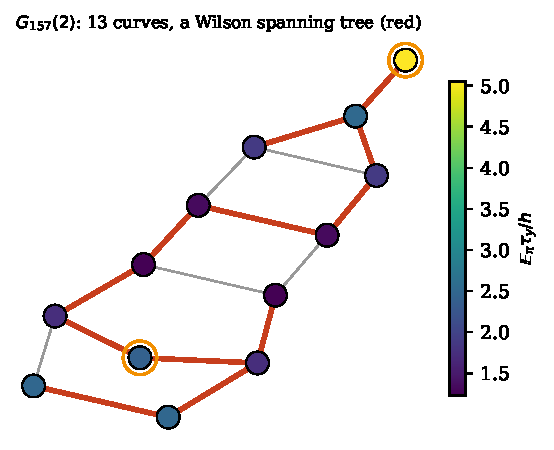
\includegraphics[width=0.72\textwidth]{figs/hit_graph.pdf}
\caption{The supersingular $2$ isogeny graph $G_{157}(2)$ (edge width is multiplicity, circles mark the two curves with loops), coloured by $\E_\pi\tau_y/h$ (Proposition~\ref{prop:hitvertex}), with a uniform spanning tree sampled by Wilson's algorithm in red. The graph has $|J_0(157)(\mathbb F_2)|/13=1418$ spanning trees.}\label{fig:hitgraph}
\end{figure}

\subsection{Data}

We built the isogeny walks from modular polynomials over $\mathbb F_{N^2}$, as in Section~\ref{sec:B:ssgraph}, for $\ell\in\{2,3,5,7\}$, the $49$ primes $N\equiv1\bmod12$ below $1300$, and the nine primes $11,23,43,47,59,71,83,107,131$, which are not $1$ modulo $12$, and computed $T_\ell$ on $S_2(\Gamma_0(N))$ independently with modular symbols in PARI/GP. Kemeny's constant of the walk, computed from the spectrum of $P$, agrees with the sum in Theorem~\ref{thm:hitkemeny} to relative error below $2\cdot10^{-14}$ in all $228$ cases with $g\ge1$, including the levels with extra automorphisms; computed in rational arithmetic from the Laplacian, it equals the sum exactly in the $108$ cases with $N\equiv1\bmod12$ below $700$. In all $196$ cases with $N\equiv1\bmod12$ the exact integer determinant of the reduced Laplacian times $h$ equals $|J_0(N)(\mathbb F_\ell)|$, computed as the characteristic polynomial of $T_\ell$ evaluated at $\ell+1$; the largest, for $N=1297$ and $\ell=7$, has $94$ digits. The Kirchhoff index agrees with Theorem~\ref{thm:hitresist} to $6\cdot10^{-16}$. Figure~\ref{fig:hitisogeny} shows $g^{-1}\log|J_0(N)(\mathbb F_\ell)|$ approaching the tree entropy, from above for $\ell=5$ and $7$; for $\ell=2$ three of the $48$ levels with $g\ge2$, and for $\ell=3$ eight, lie below it, by at most $0.02$. At $N=1297$ the values are $0.8566$, $1.2249$, $1.6973$ and $2.0187$.

\begin{figure}[t]
\centering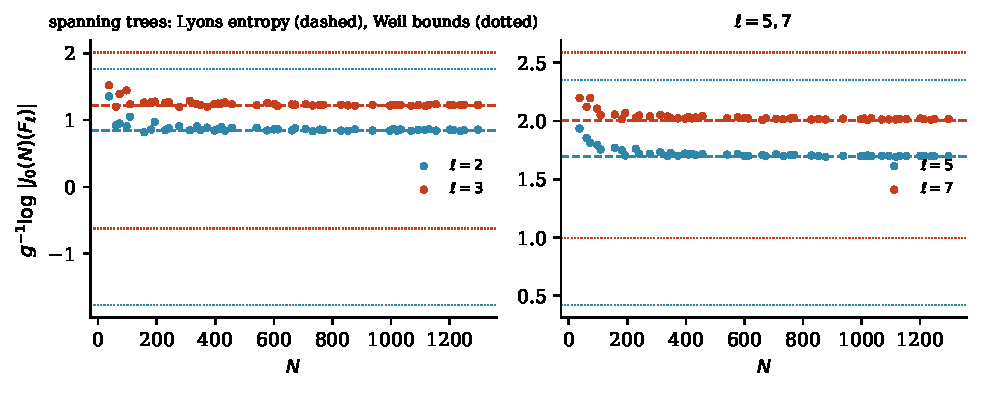
\includegraphics[width=\textwidth]{figs/hit_isogeny.pdf}
\caption{Theorems~\ref{thm:hittrees} and \ref{thm:hitentropy}: $g^{-1}\log|J_0(N)(\mathbb F_\ell)|$, which equals $g^{-1}\log(h\,\tau(G_N(\ell)))$, for primes $N\equiv1\bmod12$ below $1300$, against the spanning tree entropy of the $(\ell+1)$ regular tree (dashed) and the Weil bounds $2\log(\sqrt\ell\pm1)$ (dotted).}\label{fig:hitisogeny}
\end{figure}

\section{Chebotarev densities are hitting rates}\label{sec:hitrate}

Return to the zeta random integer $N_\sigma$ of Section~\ref{sec:recipgammaproc}, with prime factors labelled by Frobenius classes or Satake parameters $\theta_p\in Y$, equidistributed with respect to $\mu$. Scan the prime factors from the largest down. For a Borel set $B\subset Y$ let $P_B^+$ be the largest prime factor of $N_\sigma$ with label in $B$, and $V_B=(\sigma-1)\log P_B^+$ ($V_B=0$ if there is none). Write $E_1(v)=\int_v^\infty e^{-x}x^{-1}dx$ for the exponential integral.

\begin{theorem}[hitting rates; after Lloyd \cite{lloyd1984}]\label{thm:hitrate}
Let $B$ be a $\mu$ continuity set. As $\sigma\downarrow1$:
\begin{enumerate}
\item[(i)] $\Prob(V_B\le v)\to\exp(-\mu(B)E_1(v))$ for every $v>0$; if $\mu(B)>0$, equivalently, $E_1(V_B)$ converges in law to the exponential law with rate $\mu(B)$, and if $\mu(B)=0$, then $V_B\to0$ in probability;
\item[(ii)] the label of the largest prime factor of $N_\sigma$ lies in $B$ with probability tending to $\mu(B)$, and the labels of the $k$ largest prime factors are asymptotically independent with law $\mu$, independent of their sizes;
\item[(iii)] for two continuous functions $a$ and $b$ on $Y$, such as the characters $\chi_\rho$ and $\chi_{\rho'}$ of Theorem~\ref{thm:recipthorin}(a), whose discrepancy set $D=\{a\ne b\}$ is a $\mu$ continuity set, (i) holds for $B=D$, and $\mu(D)$ is the mass of the Thorin measure $\tau_Q$ of Theorem~\ref{thm:recipggcfun} for $Q=|a-b|^2$; in particular $V_D\to0$ in probability if and only if $\tau_Q=0$.
\end{enumerate}
\end{theorem}

\begin{proof}
By Theorem~\ref{thm:recipgammaproc}(i) the rescaled sizes and labels of the prime factors converge to the Poisson process with intensity $x^{-1}e^{-x}dx\otimes\mu$. Prime factors with $e_p\ge2$ give no point above a fixed level $v>0$ in the limit, since $\sum_{e\ge2}\sum_{p^e>\exp(v/(\sigma-1))}p^{-e\sigma}\to0$, so the points $((\sigma-1)\log p,\theta_p)$ have the same limit. The event $\{V_B\le v\}$ is the event that this process has no point in $(v,\infty)\times B$, whose mean number of points is $\mu(B)E_1(v)$; points beyond a large level $M$ are excluded with probability at least $1-E_1(M)-o(1)$, uniformly in $\sigma$, because the expected number of prime factors $p$ of $N_\sigma$ with $(\sigma-1)\log p>M$ is at most $\sum_{(\sigma-1)\log p>M}p^{-\sigma}(1-p^{-\sigma})^{-1}\to E_1(M)$. This gives (i), and (ii) follows from the independence of labels and sizes in the limiting Poisson process. For (iii) apply (i) to $B=D$; the Thorin mass is $\mu(D)$ by Theorem~\ref{thm:recipggcfun}.
\end{proof}

So Chebotarev's density is literally a hitting rate: in the logarithmic integral scale $E_1$, the first prime factor (from the top) whose Frobenius lies in $C$ arrives after an exponential time with rate $|C|/|G|$. Reciprocity laws are statements that a discrepancy set is hit at rate zero. For a prime $q\equiv3\bmod4$, omitting the factor $(\frac{-1}p)$ from quadratic reciprocity gives a discrepancy set that is hit at rate $\frac12$; the pair $(\rho,\rho_{31})$ of $S_3$ representations of Chapter~\ref{ch:recip} has discrepancy rate $\frac{11}{18}$.

For the $S_3$ field of $x^3-x-1$ the probability that the largest prime factor of $N_\sigma$ outside the set $S=\{2,7,11,23,31,37\}$ of the example after Theorem~\ref{thm:recipdrift} has Frobenius in a given class, conditional on there being such a factor, was computed exactly from the primes below $10^7$, with larger primes from the prime number theorem (at $\sigma=1.005$ the largest prime factor exceeds $10^7$ with probability $0.87$, and its class is then given the limit law). At $\sigma=1.005$ it is $0.1626$, $0.5000$ and $0.3375$ for the identity, the transpositions and the three cycles, against $\frac16$, $\frac12$, $\frac13$; at $\sigma=1.5$ it is $0.021$, $0.392$ and $0.587$, so at moderate $\sigma$ small primes still dominate (Figure~\ref{fig:hitrates}). To first order the approach is linear in $\sigma-1$, with slope $s_C=\sum_{p\notin S}\bigl(\mathsf 1_C(\Frob_p)-\mu(C)\bigr)p^{-1}\prod_{p'\le p\text{ or }p'\in S}(1-1/p')^{-1}$, a Chebotarev bias weighted by Mertens products; for the primes below $10^7$, $s_C=-0.835$, $0.003$ and $0.832$, so the transpositions converge fastest. For Chebotarev labels and a uniform random integer below $x$, the class of a size biased prime factor approaches Haar measure at rate $1/\log x$, the class of the largest one faster still, but the classes of the distinct prime factors only at rate $1/\log\log x$ (Chapter~\ref{ch:pd}).

\begin{figure}[t]
\centering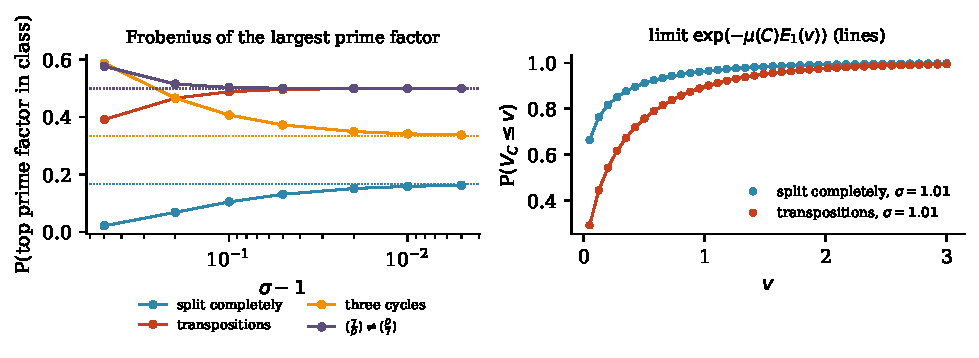
\includegraphics[width=0.72\textwidth,trim=0 0 234 0,clip]{figs/hit_rates.pdf}
\caption{Theorem~\ref{thm:hitrate} for the $S_3$ field of $x^3-x-1$: the probability that the largest prime factor of $N_\sigma$ outside $S$ has Frobenius in a given class, conditional on one existing, and that it lies in the discrepancy set $\{p:(\frac7p)\ne(\frac p7)\}$, against $\sigma-1$, with their limits (dotted).}\label{fig:hitrates}
\end{figure}

\section{Explosion times and the Thorin converse theorem}\label{sec:hitexplosion}

A pure birth process on $\{0,1,2,\dots\}$ started at $0$ with rates $u_1\le u_2\le\dots$, repetitions allowed, spends independent exponential times with means $1/u_k$ in successive states. If $\sum_k1/u_k<\infty$ it explodes at the finite time
\[
T=\sum_k\frac{\mathcal E_k}{u_k},\qquad \E e^{-sT}=\prod_k\Bigl(1+\frac s{u_k}\Bigr)^{-1},
\]
with $\mathcal E_k$ independent standard exponentials. So explosion laws are exactly the GGCs with zero drift whose Thorin measure is a sum of unit point masses: atomic Thorin measures with \emph{integer} masses. This is the integrality condition in Theorem~\ref{thm:recipeuler}, now with a meaning: multiplicities of zeros are repeated birth rates.

\begin{theorem}[explosion times; after Theorem~\ref{thm:10dduality}]\label{thm:hitexplosion}
Let $\Lambda(s)$ be entire of order at most one with $\Lambda(s)=\Lambda(1-s)$ and $\Lambda(\frac12)\ne0$, and write its zeros as $\frac12\pm i\gamma_k$, with multiplicity. The following are equivalent.
\begin{enumerate}
\item[(i)] Every $\gamma_k$ is real.
\item[(ii)] There is a generalized gamma convolution $T$ with $\E e^{-sT}=\Lambda(\frac12)/\Lambda(\frac12+\sqrt s)$ for all $s>\frac14$.
\item[(iii)] $\Lambda(\frac12)/\Lambda(\frac12+\sqrt s)$, $s>\frac14$, is the Laplace transform of the explosion time of a pure birth process.
\end{enumerate}
In that case the birth rates are the $\gamma_k^2$, $T$ is infinitely divisible with L\'evy density $\mathcal W(x)/x$, where $\mathcal W(x)=\sum_{\gamma_k>0}e^{-x\gamma_k^2}$ is the heat trace, and the cumulants of $T$ are
\[
\begin{gathered}
\kappa_m(T)=(m-1)!\sum_k\gamma_k^{-2m}=\int_0^\infty x^{m-1}\mathcal W(x)\,dx,\\
\E T=\sum_k\frac1{\gamma_k^2}=\frac12\,\frac{\Lambda''}{\Lambda}\Bigl(\frac12\Bigr).
\end{gathered}
\]
\end{theorem}

\begin{proof}
For real $\Lambda$ with $\Lambda(\frac12)>0$, the equivalence of (i) and (ii) and the Thorin measure $\sum_k\delta_{\gamma_k^2}$ are Theorem~\ref{thm:10dduality} with $f=\Lambda$ and $\alpha=\frac12$, and the variable in (iii) is that of Theorem~\ref{thm:10babstract}(c); the argument is short, and we repeat it without these hypotheses. By Hadamard, $\Lambda(\frac12+z)/\Lambda(\frac12)$ is an even entire function of order at most one, so it equals $\prod_k(1+z^2/\gamma_k^2)$ with $\sum|\gamma_k|^{-2}<\infty$, the exponential factor being trivial by evenness. If (i) holds, (iii) holds with rates $\gamma_k^2$, and an explosion time is a GGC with Thorin measure $\sum_k\delta_{\gamma_k^2}$, so (iii) implies (ii). Conversely let $T$ be a GGC with drift $a$ and Thorin measure $\tau$ as in (ii). Taking logarithms and differentiating in $s$,
\[
a+\int\frac{\tau(dt)}{t+s}=\sum_k\frac1{\gamma_k^2+s},\qquad s>\tfrac14 .
\]
The left side is analytic on $\C\setminus(-\infty,0]$, and the right side is meromorphic on $\C$ with a pole at each $-\gamma_k^2$. So every $\gamma_k^2$ lies in $[0,\infty)$, and $\gamma_k^2\ne0$ because $\Lambda(\frac12)\ne0$: every $\gamma_k$ is real. (Letting $s\to\infty$ shows $a=0$, and comparing residues shows $\tau=\sum_k\delta_{\gamma_k^2}$, as in Theorem~\ref{thm:recipeuler}.) For the L\'evy density, Frullani's integral gives $\sum_k\log(1+s/\gamma_k^2)=\int_0^\infty(1-e^{-sx})\mathcal W(x)x^{-1}dx$. The cumulants follow by differentiating at $s=0$, or from $\int_0^\infty x^{m-1}e^{-x\gamma^2}dx=(m-1)!\gamma^{-2m}$, and $\Lambda''/\Lambda(\frac12)=2\sum_k\gamma_k^{-2}$ from the product.
\end{proof}

The hypothesis in (ii) cannot be weakened to positivity of $T$. With $w=2+i$, the function $1/((1+s)(1+s/w)(1+s/\bar w))$ is the Laplace transform of the probability density $\frac52e^{-t}\bigl(1-e^{-t}(\cos t+\sin t)\bigr)$ on $(0,\infty)$, which is nonnegative because $e^{-t}(\cos t+\sin t)$ decreases on $[0,\pi]$ and is at most $\sqrt2e^{-\pi}<1$ beyond, although two of its poles are not real. What the GGC property adds is positivity of the Thorin measure, which forces the poles onto the negative axis.

The mean explosion time is a number computed from Galois data. By Definition~\ref{def:recipheat} the heat trace $\mathcal W$ is given by the explicit formula from the prime powers, the conductor and the gamma factor, and $\E T=\int_0^\infty\mathcal W(x)\,dx$. Under GRH this integral is the mean of a positive random variable, the explosion time whose birth rates are the squared ordinates $\gamma_k^2$ of the zeros. For $\xi$, for $L(s,\Delta)$ in the unitary normalisation and for the $S_3$ representation $\rho$ of $x^3-x-1$, of conductor $23$, the sum $\sum_k\gamma_k^{-2}$ is the constant $S_1$ of Table~\ref{tab:10bcatalogue}, $0.023105$, $0.0561759$ and $0.170287$, computed there from the central Taylor coefficients and checked against the zeros.

The mean explosion time can also be computed from the Frobenius classes, the conductor and the gamma factor, with no analytic continuation; only the tail of the integral needs a bound on the zeros. For the $S_3$ representation $\rho$ we evaluated the Galois heat trace of Definition~\ref{def:recipheat} from the Frobenius classes of $x^3-x-1$ at the $664579$ primes below $10^7$ and their powers below $10^7$, with the archimedean integral by quadrature. It agrees with $\sum e^{-x\gamma^2}$ over the zeros to fifteen digits at $x=0.001$, $0.005$, $0.02$ and $0.1$. Integrating over $e^{-60}\le x\le1.1$ (beyond which $\mathcal W<e^{-28}$, by the first zero $\gamma_1=5.1157$) gives
\[
\int_{e^{-60}}^{1.1}\mathcal W(x)\,dx=0.17028731076215,
\]
against $0.17028731076373$ from the Hadamard product, a difference of $1.6\cdot10^{-12}$ that the integral over the two omitted ends accounts for to $3\cdot10^{-17}$. Since $L(s,\rho)$ is entire, $\rho$ being dihedral, the explicit formula gives $\mathcal W(x)=\sum_ke^{-x\gamma_k^2}$ unconditionally. If GRH holds for $L(s,\rho)$, which is not known, $\sum_k\gamma_k^{-2}$ is the mean explosion time of a birth process whose rates are the squared ordinates of the zeros, and it has been computed from the factorisation of $x^3-x-1$ modulo primes (which determines the Frobenius class in $S_3$), the conductor $23$ and the gamma factor. The agreement does not verify GRH: a finite computation of this kind can disprove it and is not known to verify it.

Combining Theorem~\ref{thm:hitexplosion} with Corollary~\ref{cor:recipconverse} gives an explosion form of the Thorin converse theorem.

\begin{corollary}[Thorin converse theorem as explosion; this book]\label{cor:hitconverse}
Let $k\equiv0\bmod4$ and let $(a_p)$ be the Frobenius traces of a self dual Galois representation of conductor $1$ with the gamma factor $\Gamma_\C(s+\frac{k-1}2)$ of Corollary~\ref{cor:recipconverse} and the Ramanujan bound, and $\Lambda$ its completion, defined on $\operatorname{Re}s>1$ by the Euler product. If for some constant $c>0$ the function $c/\Lambda(\frac12+\sqrt s)$, $s>\frac14$, is the Laplace transform of the explosion time $T$ of a pure birth process, then $f=\sum a_nn^{(k-1)/2}q^n$ is a cusp form for $\SL_2(\Z)$ satisfying GRH, and $c=\Lambda(\frac12)\ne0$. Conversely, if $f$ is such a cusp form satisfying GRH with $\Lambda(\frac12)\ne0$, this holds with $c=\Lambda(\frac12)$. If moreover the P\'olya kernel $\Phi_f$ is nonnegative, as for $\Delta$ (but not for one of the two eigenforms of weight $24$), then the P\'olya variable $W_f$ and $T$ form a Wald couple: $\E e^{tW_f}\,\E e^{-t^2T}=1$ for all real $t$.
\end{corollary}

\begin{proof}
Explosion laws are exactly the GGCs with integer atomic Thorin measures. Under the hypothesis, $\Lambda(\frac12+\sqrt{s_0})/\Lambda(\frac12+\sqrt s)$ is $c^{-1}\Lambda(\frac12+\sqrt{s_0})$ times the Laplace transform of such a GGC, so Corollary~\ref{cor:recipconverse} gives the cusp form and GRH; then $\Lambda(\frac12+z)=c\prod_k(1+z^2/u_k)$ and $z=0$ gives $c=\Lambda(\frac12)$. The converse is Theorem~\ref{thm:hitexplosion}. For the Wald couple, $\E e^{tW_f}=\Lambda(\frac12+t)/\Lambda(\frac12)$ for every real $t$, by \eqref{eq:recipmellin} (whose classical completion at $\frac k2+t$ is a constant times $\Lambda(\frac12+t)$) and the doubly exponential decay of $\Phi_f$, and $\E e^{-t^2T}=\prod_k(1+t^2/\gamma_k^2)^{-1}=\Lambda(\frac12)/\Lambda(\frac12+t)$ by the Hadamard product; this is the Wald couple of Theorem~\ref{thm:10dvdp}(c).
\end{proof}

As with Corollary~\ref{cor:recipconverse}, the hypothesis contains GRH, so it is stronger than reciprocity. Keilson's theorem (Theorem~\ref{thm:10ckeilson}) and Kent's extension to diffusions \cite{kent1980} go the other way: first passage times of birth death chains and of diffusions have laws of this form, with rates from their spectra, and whether a given law is such a passage time is an inverse spectral question. The pure birth realisation needs no simplicity of the zeros and is the one that matches the integrality in the Thorin converse theorem.

\section{Brownian exit and the functional equation of odd characters}\label{sec:hitexit}

The functional equations of even Dirichlet $L$ functions came in Section~\ref{sec:recipgauss} (Theorem~\ref{thm:recipdirichlet}) from the wrapped normal law. For odd characters the natural object is the exit of Brownian motion from an interval, and the signed starting distribution is the character itself.

Let $q\ge3$, let $B$ be standard Brownian motion started at $r\in(0,q)$, let $\tau$ be its exit time from $(0,q)$, and let $f_r^0(t)$ and $f_r^q(t)$ be the densities of $\tau$ on the events of exit at $0$ and at $q$.

\begin{theorem}[signed exit law; after Biane, Pitman and Yor \cite{bpy2001}]\label{thm:hitexit}
Let $\chi$ be an odd primitive character modulo $q$ and $g(\chi)=\sum_r\chi(r)e^{2\pi ir/q}$. For every $t>0$,
\[
\begin{split}
\sum_{r=1}^{q-1}\chi(r)\bigl(f_r^0(t)-f_r^q(t)\bigr)&=\frac2{\sqrt{2\pi t^3}}\sum_{m\ge1}\chi(m)\,m\,e^{-m^2/(2t)}\\
&=-\frac{4\pi i\,g(\chi)}{q^2}\sum_{j\ge1}\bar\chi(j)\,j\,e^{-2\pi^2j^2t/q^2}.
\end{split}
\]
Consequently $\vartheta_\chi(x)=\sum_{n\ge1}\chi(n)\,n\,e^{-\pi n^2x/q}$ satisfies
\[
\vartheta_\chi(1/x)=\frac{g(\chi)}{i\sqrt q}\,x^{3/2}\,\vartheta_{\bar\chi}(x),
\]
and $\Lambda(s,\chi)=(q/\pi)^{(s+1)/2}\Gamma(\frac{s+1}2)L(s,\chi)$ satisfies $\Lambda(s,\chi)=\frac{g(\chi)}{i\sqrt q}\Lambda(1-s,\bar\chi)$.
\end{theorem}

\begin{proof}
The method of images (the reflection principle) gives
\[
\begin{aligned}
f_r^0(t)&=\sum_{n\in\Z}\frac{r+2nq}{\sqrt{2\pi t^3}}e^{-(r+2nq)^2/(2t)},\\
f_r^q(t)&=\sum_{n\in\Z}\frac{q-r+2nq}{\sqrt{2\pi t^3}}e^{-(q-r+2nq)^2/(2t)} .
\end{aligned}
\]
In the first sum $m=r+2nq$ runs over the integers $\equiv r\bmod 2q$ and $\chi(r)=\chi(m)$. In the second $m=q-r+2nq\equiv-r\bmod q$, so $\chi(r)=-\chi(m)$ because $\chi$ is odd. Hence $\sum_r\chi(r)(f_r^0-f_r^q)=2(2\pi t^3)^{-1/2}\sum'\chi(m)me^{-m^2/2t}$, the sum over all integers $m$ whose residue modulo $2q$ lies in $(0,q)$. For negative $m$ put $m'=-m$; then $m'\bmod2q\in(q,2q)$ and $\chi(m)m=\chi(m')m'$. The two ranges together cover every positive integer prime to $q$ once, which is the first identity. The eigenfunction expansion of the killed heat kernel gives
\[
f_r^0(t)-f_r^q(t)=\sum_{k\ge1}\frac{k\pi}{q^2}\bigl(1+(-1)^k\bigr)\sin\frac{k\pi r}q\,e^{-k^2\pi^2t/(2q^2)},
\]
since exit at $q$ from $r$ is exit at $0$ from $q-r$, and $\sin(k\pi(q-r)/q)$ equals $(-1)^{k+1}\sin(k\pi r/q)$. Only $k=2j$ survives, and for odd primitive $\chi$,
\[
\sum_r\chi(r)\sin\frac{2\pi jr}q=\frac1{2i}\bigl(\bar\chi(j)-\bar\chi(-j)\bigr)g(\chi)=-i\,\bar\chi(j)g(\chi).
\] This is the second identity. Putting $t=qx/(2\pi)$ and comparing gives the transformation of $\vartheta_\chi$, and the Mellin transform $\int_0^\infty\vartheta_\chi(x)x^{(s+1)/2}dx/x=\Lambda(s,\chi)$ gives the functional equation in the usual way.
\end{proof}

The root number $g(\chi)/(i\sqrt q)$ is the eigenfunction weight of the signed starting law, the Fourier coefficient of $r\mapsto\chi(r)$ against the sine modes of the interval. For a real odd character modulo a prime $q\equiv3\bmod4$ it is $1$, which is Gauss's sign $g(\chi)=g(q)=i\sqrt q$ of Corollary~\ref{cor:recipgausssign}. For $q=4$, $\chi=\chi_{-4}$, the theorem is the reciprocal law of the exit time of Brownian motion started at the centre of an interval, which Biane, Pitman and Yor \cite{bpy2001} credit to Ciesielski and Taylor \cite{ciesielskitaylor1962} and from which they obtained the functional equation of Dirichlet's $\beta$ function; Salminen and Vignat \cite{salminenvignat2024} derive it by comparing the image and eigenfunction expansions, as here. For real odd characters Biane, Pitman and Yor wrote the Laplace transform of $\vartheta_\chi$, using the classical transformation formula, as a combination with weights $\chi(n)$ of ratios of hyperbolic sines, which are Laplace transforms of Brownian exit laws from an interval, and observed, after P\'olya, that $\vartheta_\chi$ need not be positive, while its positivity would exclude a real zero of $L(s,\chi)$ (\cite{bpy2001}, Section~6.1). Theorem~\ref{thm:hitexit} reads that combination as an exit law whose starting point is spread over the interval with the character as a signed weight, and reverses the argument: the transformation formula follows by comparing the image and eigenfunction expansions. For $\chi_{-4}$ the function $\vartheta_\chi$ is positive, since $\vartheta_{\chi_{-4}}(x)=\eta(ix)^3$ by Jacobi's identity (Proposition~\ref{beta:prop:kernel}). For the character $\chi_d$ of an imaginary quadratic field $K$ of discriminant $d$, the completed Dedekind zeta function of $K$ is a constant multiple of $\xi(s)\Lambda(s,\chi_d)$, so its P\'olya kernel (Theorem~\ref{thm:sf:kernel}) is a positive multiple of the convolution of P\'olya's kernel of $\xi$ with $v\mapsto e^{3v/2}\vartheta_{\chi_d}(e^{2v})$; hence, by Theorem~\ref{thm:sf:inert}, $\vartheta_{\chi_d}$ takes negative values whenever $2$ and $3$ are inert in $K$, that is whenever $d\equiv5\bmod24$. In $40$ digit arithmetic, for $\chi_{-3}$, $\chi_{-4}$, $\chi_{-7}$, $\chi_{-8}$, the odd character modulo $5$ with $\chi(2)=i$ and an odd character of order $6$ modulo $7$ at $t=0.3$, $1$ and $3$, the image and eigenfunction sums agree with each other and with both closed forms to $10^{-40}$; Figure~\ref{fig:hitexit} plots four of these characters.

\begin{figure}[t]
\centering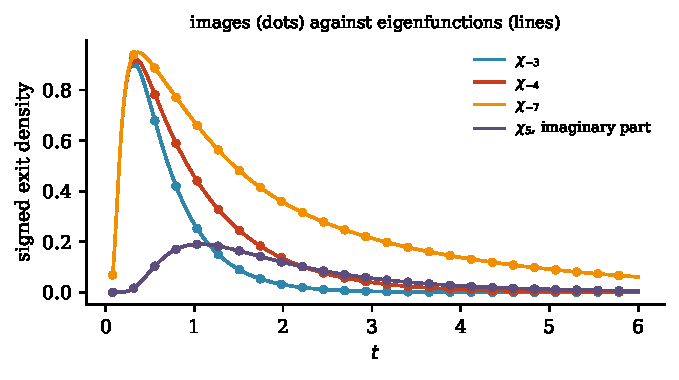
\includegraphics[width=0.72\textwidth]{figs/hit_exit.pdf}
\caption{Theorem~\ref{thm:hitexit} for $\chi_{-3}$, $\chi_{-4}$, $\chi_{-7}$ and the odd character modulo $5$ with $\chi(2)=i$ (imaginary part, labelled $\chi_5$): the two closed forms of the signed exit density, the image sum (dots) and the eigenfunction sum with the Gauss sum as weight (lines).}\label{fig:hitexit}
\end{figure}

\section{A dictionary}\label{sec:hitdictionary}

The correspondences of the chapter, side by side.

\begin{center}\small
\begin{tabular}{p{0.44\textwidth}p{0.46\textwidth}}
\toprule
Hitting time & Reciprocity\\
\midrule
Kemeny constant of the isogeny walk mod $N$ & harmonic sum of the factors $\ell+1-a_\ell(f)$ of $|J_0(N)(\mathbb F_\ell)|$\\
spanning trees ($N\equiv1\bmod12$) & $|J_0(N)(\mathbb F_\ell)|/|J_0(N)(\Q)_{\mathrm{tors}}|$\\
critical group ($N\equiv1\bmod12$) & order $|J_0(N)(\mathbb F_\ell)|/h$; $r$ part $\mathbb T_r/(\ell+1-T_\ell)\mathbb T_r$ for $r\nmid\ell hN$ prime to the discriminant of $\mathbb T$ (Proposition~\ref{prop:hitsandpile})\\
tree entropy of $\T_\ell$ & growth of $|J_0(N)(\mathbb F_\ell)|$\\
bounds on hitting times and spanning trees & Weil bound for $a_\ell(f)$\\
hitting rate of a class by top prime factors & Chebotarev density\\
discrepancy set hit at rate zero & reciprocity, vanishing Thorin mass\\
explosion time of a pure birth process & Thorin converse theorem, GRH\\
mean explosion time & $\int\mathcal W$, computable from Frobenius data, conductor and gamma factor\\
signed exit law, images against eigenfunctions & functional equation of odd $L(s,\chi)$\\
\bottomrule
\end{tabular}
\end{center}

\subsection{Open problems}

\begin{problem}[Sandpile groups and Jacobians]\label{op:hitsandpile}
Fix $\ell$ and let $N\to\infty$ through primes $N\equiv1\bmod12$. Find the limiting law of the $r$ part of the critical group of $G_N(\ell)$, a question Munier and Shnidman raise \cite{muniershnidman2023}. By Proposition~\ref{prop:hitsandpile}, for $r\ne\ell$ prime to $hN$ and to the discriminant of $\mathbb T$, it is governed by the valuations of $\ell+1-a_\ell(f)$ at the primes above $r$ of the Hecke fields, so, as Munier and Shnidman note, it needs an $r$ adic analogue of the vertical equidistribution of Theorem~\ref{thm:07serre}. For the primes $r$ dividing $h$ or the discriminant of $\mathbb T$, which Proposition~\ref{prop:hitsandpile} excludes, describe the critical group, and decide when the class of $L\delta_E$ corresponds to the cuspidal subgroup $C_N$. Extend the comparison to $\ell=2$ and to levels $N\not\equiv1\bmod12$, where the graph is weighted by automorphisms.
\end{problem}

\begin{problem}[Vertex hitting times and Gross's formula]\label{op:hitgross}
By Exercise~\ref{ex:hitgross}, Gross's formula turns the mean $\sum_{x,y}c_xc_y\E_x\tau_y$ of hitting times between the reductions of the curves with complex multiplication by discriminant $D$, less its stationary part $(\deg e_D)\sum_yc_y\E_\pi\tau_y$, into a combination of the central values $L(f,1)L(f\otimes\chi_D,1)$ over the newforms of level $N$. For fixed $N$ and $\ell$, find the distribution of this combination over $D$, a question about the central values of the quadratic twists of the newforms of level $N$. Find also the law of the hitting time of the support of $e_D$ from stationarity, and decide which arithmetic quantities it computes: its Laplace transform involves the values $\phi_f(x)\overline{\phi_f(y)}$ at pairs of points of the support, not only the linear forms $\sum_yc_y\phi_f(y)$ of Gross's formula.
\end{problem}

\section{Notes}

The supersingular isogeny graph and Brandt matrices are in Deuring, Eichler, Mestre, Gross and Pizer \cite{deuring1941,eichler1954,mestre1986,gross1987,pizer1990}; the congruence relation is Eichler and Shimura \cite{shimura1971}; rational torsion of $J_0(N)$ is Ogg's conjecture proved by Mazur \cite{ogg1975,mazur1977}, and injectivity of reduction on torsion is in Katz \cite{katz1981}. Kemeny's constant is from \cite{kemenysnell1960}, the matrix tree theorem is Kirchhoff's \cite{kirchhoff1847}, critical groups are in Biggs \cite{biggs1997} and Baker and Norine \cite{bakernorine2007}, uniform spanning trees from random walks in Aldous, Broder and Wilson \cite{aldous1990,broder1989,wilson1996}, resistances in Doyle and Snell \cite{doylesnell1984}, the Kirchhoff index in \cite{gutmanmohar1996,zhukleinlukovits1996} and the commute time identity in \cite{chandra1996}. McKay \cite{mckay1983} computed the asymptotic number of spanning trees of regular graphs with large girth and Lyons \cite{lyons2005} the tree entropy. The vertical Sato Tate theorem is Serre's \cite{serre1997}. Explosion of pure birth processes is classical (Feller \cite{feller1968}, Section XVII.4), Keilson's theorem is \cite{keilson1971}, Kent's is \cite{kent1980}. The tree count of Theorem~\ref{thm:hittrees} is Hashimoto's formula \cite[(7.14)]{hashimoto1989}, presented by Li \cite[Section~4.3]{li2019}; Munier and Shnidman \cite{muniershnidman2023} sketch the proof given here, call the formula a kind of reciprocity law between the Jacobian of the graph and that of $X_0(N)$, prove Proposition~\ref{prop:hitcritical} and the first statement of Proposition~\ref{prop:hitsandpile}, note the cuspidal point behind Corollary~\ref{cor:hittorsion}, and find the laws of the $r$ parts of the critical groups for fixed $N$ and $r\nmid6h$ prime to the discriminant of $\mathbb T$, as $\ell\to\infty$. The limit in Theorem~\ref{thm:hitentropy} is an asymptotic class number of Tsfasman and Vl\u{a}du\c{t} \cite{tsfasmanvladut2002}. For one label, Theorem~\ref{thm:hitrate}(i) is Lloyd's limit law for the largest prime factor \cite{lloyd1984}, and Theorem~\ref{thm:hitexplosion} restates Theorems~\ref{thm:10babstract} and \ref{thm:10dduality}. Theorem~\ref{thm:hitexit} is after Biane, Pitman and Yor \cite{bpy2001}, as explained after it, and the transformation formula is classical (\cite{bump1997}, Section~1.1). Deriving theta transformations from the heat equation goes back at least to Bellman \cite{bellman1961}, for $\vartheta_3$, and Salminen and Vignat \cite{salminenvignat2024} derive the modular identities of the Jacobi theta functions by comparing the image and eigenfunction expansions of the heat kernels of an interval, among them the case $q=4$ of Theorem~\ref{thm:hitexit}, the exit time from the centre. Ours are Theorems~\ref{thm:hitkemeny} and \ref{thm:hitresist} in the forms stated (for $N\equiv1\bmod12$ the Kemeny formula is the expression in the proof of Theorem~\ref{thm:08kemeny}), the isomorphism criterion of Proposition~\ref{prop:hitsandpile}, the reading of the limit in Theorem~\ref{thm:hitentropy} as a tree entropy, the labelled form of Theorem~\ref{thm:hitrate}, the explosion reading of Theorem~\ref{thm:hitexplosion}, the extension of the image and eigenfunction derivation to every odd primitive character through the signed exit law of Theorem~\ref{thm:hitexit}, Corollaries~\ref{cor:hithasse} and \ref{cor:hitconverse}, and the computations; each is a short consequence of the cited theory, and none proves a new case of reciprocity, of Artin's conjecture or of GRH.

\section{Exercises}

\begin{enumerate}
\item Compute $G_{11}(2)$ and $G_{11}(3)$ from $\Phi_2$ and $\Phi_3$ over $\mathbb F_{121}$, with the weights $w$ of $j=0$ and $j=1728$, and check $K_{11}(2)=\frac35$, $K_{11}(3)=\frac45$ against $|11a1(\mathbb F_2)|=|11a1(\mathbb F_3)|=5$.
\item For $N=37$ and $\ell=2$, draw the three vertex graph, list its five spanning trees and compute all hitting times. Compare with Proposition~\ref{prop:hitvertex}.
\item Show that the Laplace transform of the explosion time of a pure birth process determines the multiset of rates, and deduce that Corollary~\ref{cor:hitconverse} recovers the zeros with multiplicity.
\item Check Theorem~\ref{thm:hitexit} for $\chi_{-3}$ by computing the image sum and the eigenfunction sum at $t=1$ to ten digits, verify $g(\chi_{-3})=i\sqrt3$, and derive the functional equation of $L(s,\chi_{-3})$ from the transformation of $\vartheta_{\chi_{-3}}$.
\item Show that $\E[(\sigma-1)\log P^+(N_\sigma)]\to\int_0^\infty x\cdot\frac{d}{dx}e^{-E_1(x)}dx$, where $P^+$ is the largest prime factor ($P^+(1)=1$), and that the limit is the Golomb Dickman constant $\int_0^\infty e^{-x-E_1(x)}dx=0.62433\ldots$ (Lloyd \cite{lloyd1984}; for uniform integers, Theorem~\ref{thm:pdbillingsley}). To pass from convergence in law to convergence of means, bound $\E[V;V>M]$, for $V=(\sigma-1)\log P^+(N_\sigma)$, by the expected sum of $(\sigma-1)\log p$ over the prime factors $p$ with $(\sigma-1)\log p>M$, which tends to $e^{-M}$.
\item\label{ex:hitgross} Let $N\equiv1\bmod12$, let $D<0$ be a fundamental discriminant with $N$ inert in $\Q(\sqrt D)$, and let $e_D=\sum_yc_y[E_y]$ be the divisor of Gross's formula \cite{gross1987}, whose coefficient $c_y$ counts the curves with complex multiplication by the ring of integers of $\Q(\sqrt D)$ that reduce to $E_y$. With $\phi_f$ as in Proposition~\ref{prop:hitvertex}, show that
\[
\sum_{x,y}c_xc_y\E_x\tau_y=(\deg e_D)\sum_yc_y\E_\pi\tau_y-(\ell+1)\sum_f\frac{\bigl|\sum_yc_y\phi_f(y)\bigr|^2}{\ell+1-a_\ell(f)},
\]
using $\E_x\tau_y=(Z(y,y)-Z(x,y))/\pi(y)$ (Theorem~\ref{thm:A:kemeny}), and deduce from Gross's formula that the last sum is a combination of the $L(f,1)L(f\otimes\chi_D,1)/(\ell+1-a_\ell(f))$ with positive coefficients that do not depend on $\ell$.
\item\label{ex:hitnonback} Show that the nonbacktracking walk on a connected $(q+1)$ regular graph on $n$ vertices without half loops, $q\ge2$, has Kemeny constant $(n-1)+\frac{q-1}{q+1}K+\frac q{q-1}+\frac{nq^2}{q+1}$, where $K$ is the Kemeny constant of the simple walk (use the Ihara Bass formula of Chapter~\ref{ch:08}). When $G_N(\ell)$ has no half loops, write it with Theorem~\ref{thm:hitkemeny} as a sum over the factors $\ell+1-a_\ell(f)$ of $|J_0(N)(\mathbb F_\ell)|$.
\end{enumerate}

\section{Open computational problems}

\begin{compproblem}[Two prime tables]\label{cp:hittables}
Objective: for fixed $\ell$ and small primes $r\ne\ell$, the empirical law of the $r$ part of the critical group of $G_N(\ell)$ over the primes $N\equiv1\bmod12$, against the Haar model that Munier and Shnidman prove for fixed $N$ and $\ell\to\infty$ and against the Cohen Lenstra law of Chapter~\ref{ch:06c} (Open Problem~\ref{op:hitsandpile}), with the frequency of noncyclic $r$ parts of $J_0(N)(\mathbb F_\ell)$. Objects and scale: the primes $N\equiv1\bmod12$ below $10^5$ and $\ell\le13$, with graphs of up to about $8300$ vertices. Route: for $r$ prime to $hN$ and to the discriminant of $\mathbb T$, the valuations of $\ell+1-a_\ell(f)$ in the Hecke fields (Proposition~\ref{prop:hitsandpile}), from modular symbols in PARI/GP or Magma; Smith normal forms of the reduced Laplacians for the other $r$. Deliverable: tables of the laws and of the proportion of cyclic critical groups, and the second order term $\log|J_0(N)(\mathbb F_\ell)|-g\log\frac{\ell^\ell}{(\ell^2-1)^{(\ell-1)/2}}$ of Theorem~\ref{thm:hitentropy}, which the trace formula writes formally as a series in Legendre symbols at $N$, like the Kemeny correction of Problem~\ref{cp:08second}. Why it matters: it tests a random matrix model for arithmetic critical groups in the level aspect, where no theorem is known. Kemeny constants at these degrees are Problem~\ref{cp:08second} and the problem on other degrees in Chapter~\ref{ch:08}.
\end{compproblem}

\begin{compproblem}[Explosion cumulants from Frobenius]\label{cp:hitexplosion}
Objective: for the even icosahedral representation $\rho$ of Problem~\ref{cp:recipicosa}, compute $\int_0^\infty x^{m-1}\mathcal W_\rho(x)\,dx$ for $m=1,2$ via Definition~\ref{def:recipheat}, as Section~\ref{sec:hitexplosion} does for the $S_3$ representation, from the Frobenius classes (factorisation patterns, with a Frobenius resolvent \cite{dokchitser2013} to separate the two classes of order $5$ and the two of order $10$), the conductor and the gamma factor. If $\Lambda(s,\rho)$ is entire and satisfies GRH, neither of which is known, these are $(m-1)!\sum_k\gamma_k^{-2m}$, the mean and the variance of the explosion time. Objects and scale: prime powers up to $10^{10}$, which at conductors of a few million control $\mathcal W_\rho$ only for $x$ up to about $4$ (Problem~\ref{cp:recipicosa}). Route: ball arithmetic for $x\le4$; for larger $x$, the explicit formula with the lowest zeros located numerically, since the range of $x$ grows only like $(\log P)^2$ with the prime range $P$. Deliverable: the integrals over $x\le4$ with rigorous error bounds, compared with the same integrals over the zeros, and the full integrals, whose part beyond $x=4$ rests on the computed zeros, compared with the power sums $S_1$ and $S_2$ of \eqref{eq:10bkS} computed from central derivatives as in Chapter~\ref{ch:10b}. Why it matters: it checks the Galois data against the zeros on the range that the primes control; a disagreement beyond the error bounds would point to a pole or a missed zero, while agreement verifies neither holomorphy nor GRH.
\end{compproblem}

\begin{compproblem}[Signed exit laws and real zeros]\label{cp:hitexit}
Objective: for every real odd primitive character $\chi$ of conductor $q<10^6$, decide whether the signed exit density of Theorem~\ref{thm:hitexit}, here $(4\pi/q^{3/2})\vartheta_\chi(2\pi t/q)$, is positive for all $t>0$; positivity excludes a real zero of $L(s,\chi)$ \cite{bpy2001}. For $\chi=\chi_D$ with $D\equiv5\bmod24$ the density takes negative values, by Theorem~\ref{thm:sf:inert} (Section~\ref{sec:hitexit}). Objects and scale: the characters $\chi_D$ of the fundamental discriminants $-10^6<D<0$, about $3\cdot10^5$ of them. Route: the root number is $1$, so $\vartheta_\chi(1/x)=x^{3/2}\vartheta_\chi(x)$ and it suffices to take $x\ge1$; lower bounds in ball arithmetic (Arb or PARI/GP) on a grid, with bounds on the derivative between grid points. Deliverable: the list of $D$ with positive density and their proportion in dyadic ranges of $|D|$, the first sign change for the others, and a comparison with the positivity on $(0,1)$ of the Fekete polynomial $\sum_{n<q}\chi(n)y^n$, a weaker condition implied by positivity of the density (its Laplace transform is a positive multiple of a value of this polynomial), which already fails for $q=43$ (\cite{bpy2001}, Section~6.1). Why it matters: it measures how far the Brownian route to excluding real zeros goes, and on which characters it fails first.
\end{compproblem}
